\documentclass[a4paper]{report}

% Use swiss german letters
\usepackage[utf8]{inputenc}

% Language: german
\usepackage[ngerman]{babel}

% Fancy Figures
\usepackage{graphicx}

% Use Times
\usepackage{mathptmx}

% Display the Bibliography in the TOC
\usepackage{tocbibind}

% Better lists
\usepackage{enumitem}

% We want SI units!!!
\usepackage{siunitx}

% Use biblatex
\usepackage[style=apa,backend=biber,citestyle=authoryear]{biblatex}

% Footnote glue to bottom
\usepackage[bottom]{footmisc}

% Tell BibLatex to use the ngerman language mapping
\DeclareLanguageMapping{ngerman}{ngerman-apa}

% Define the bibliography file
\addbibresource{bibliography.bib}

% To let LaTeX handle "
\usepackage[autostyle=true, german=quotes]{csquotes}

% Rename the Abstract to Management Summary
\addto\captionsngerman{\renewcommand{\abstractname}{Management Summary}}

% Titlepage
\newcommand*{\titleAP}{\begingroup % Create the command for including the title page in the document
	\centering
	\vspace*{\baselineskip} % Whitespace at the top of the page

	{\Large FirstName LastName}\\[0.167\textheight] % Author name

	{\Huge\bfseries Projektdokumentation PREN Gruppe03}\\[\baselineskip]

	%TODO review subtitle
	{\Large \textit{Subtitle}}\\
	\today

	\vspace*{3\baselineskip} % Whitespace at the bottom of the page
	\endgroup}

% Define the path were images are found
\graphicspath{{./img/}}

\begin{document}

\titleAP

\newpage

\chapter*{Redlichkeitserklärung}
% TODO Soll eig. kein Chapter sein.. und auch nicht in table of content auftauchen.
% Comments und TODOs kann man mit % einfügen - TeXStudio erkennt diese auch
% Das das Kapitel nicht im ToC erscheint eunfach ein \chapter* benutzen ;-)

\newpage

\begin{abstract}
	Hier würde man das Abstract oder Management Summary schreiben.
\end{abstract}

\tableofcontents

\newpage

\chapter{Einleitung}
\label{ch:Intro}

\chapter{Projektorganisation}

\section{Teamübersicht}

\begin{tabular}{|p{0.3\textwidth}|p{0.3\textwidth}|}
	\hline
	\textbf{Name} & \textbf{Studium} \\
	\hline
	Pascal Baumann & Informatik \\
	\hline
	Basil Bachmann & Maschinenbau \\
	\hline
	David Craven & Elektrotechnik \\
	\hline
	Victor Guntern & Maschinenbau \\
	\hline
	Markus Kempf & Maschinenbau \\
	\hline
	Eve Meier & Informatik \\
	\hline
	Jan Odermatt & Elektrotechnik \\
	\hline
	Simon Rohrer & Maschinenbau \\
	\hline
\end{tabular}

\section{Projektrollen}

\begin{tabular}{|p{0.3\textwidth}|p{0.5\textwidth}|p{0.2\textwidth}|}
	\hline
	\textbf{Rolle} & \textbf{Aufgaben} & \textbf{Teammitglied} \\
	\hline
	Projektleiter & Gesamtübersicht des Projektes halten  & Eve \\
	& Überprüfen ob Vorgaben eingehalten werden & \\
	& Teammeetings organisieren & \\
	& Informationsaustausch sicherstellen & \\
	& Kostenverwaltung & \\
	\hline
	Projektplaner & Aktualisieren des Terminplanes & Markus\\
	& Rahmenplanung und Meilensteineinhaltung & \\
	& Pflege Taskboard & \\
	\hline
	Verantwortlicher& Meilensteinabgabe zusammenstellen & Pascal \\
	Dokumentation& Protokolle führen & \\
	& Unterstützung und Pflege LaTeX &  \\
	\hline
	Fachverantwortliche & Projektstand und Feedback & I Pascal \\
	& Ansprechperson bei Fragen & ET Jan\\
	& Aktualisierung Risikomanagement & M Markus\\
	& Koordination Versuche und Recherche & \\
	\hline
\end{tabular}

\section{Tools}
\begin{tabular}{|p{0.4\textwidth}|p{0.6\textwidth}|}
	\hline
	\textbf{Aufgabe} & \textbf{Hilfsmittel} \\
	\hline
	Dokumente und Dokumentation & LaTeX / MiKTeX / GitHub \\
	\hline
	Quellen & Mendeley \\
	\hline
	Dateiablage für Teamaustausch & Dropbox \\
	\hline
	Dateiablage für Abgabe & Ilias \\
	\hline
	Projekt- und Budgetplan & MS Excel 2016 \\
	\hline
	Kommunikation Team & WhatsApp Gruppe od. HSLU Mailadresse\\
	\hline
	Aufgabenverwaltung & SCRUM-angelehntes Board, physisch, Teaminsel\\
	\hline
\end{tabular}

\section{Wochenplan}
\begin{tabular}{|p{0.2\textwidth}|p{0.8\textwidth}|}
	\hline
	\textbf{Tag} & \textbf{Beschreibung} \\
	\hline
	DO 08:30 & Alle Mitglieder sind in der Teaminsel \\
	\hline
	DO 08:30-09:00 & Besprechung Team-intern erledigte Aufgaben \\
	& Fragen, weiteres Vorgehen \\
	\hline
	DO 09:00-10:00 & Arbeiten im Team od. selbständig \\
	\hline
	DO 10:00-10:20 & Pause \\
	\hline
	DO 10:20-12:00 & Arbeiten im Team od. selbstständig \\
	\hline
	FR 08:30 & Alle Mitglieder sind in der Teaminsel \\
	\hline
	FR 08:30-09:00 & Besprechung Team-intern, Vorbereitung Meeting mit Dozent \\
	\hline
	FR 09:00-09:30& Besprechung mit Dozent \\
	\hline
	FR 09:30-10:00 & Arbeiten im Team od. selbstständig \\
	\hline
	FR 10:00-10:20 & Pause \\
	\hline
	FR 10:20-11:00 & Arbeiten im Team od. selbstständig \\
	\hline
	FR 11:00-11:30 & Kurzbesprechung, Taskboard aktualisieren \\
	\hline
	FR 11:30-12:00 & Arbeiten im Team od. selbstständig (freiwillig)\\
	\hline
\end{tabular}

\section{Projektplan}
TODO Projektplan einfügen zusätzlich Terminplan mit Arbeitspaketen und Meilensteinen - Rahmenplan

\section{Budgetplan}
Für den Bau der Teilfunktionsmuster in PREN1 dürfen maximal CHF 200.- ausgegeben werden.

% TODO Stimmen diese vertikalen Spacers noch???
\vspace{1em}
\begin{tabular}{|p{0.2\textwidth}|p{0.2\textwidth}|p{0.2\textwidth}|p{0.2\textwidth}|}
	\hline
	\textbf{Artikel} & \textbf{Anzahl} & \textbf{Preis/Stk.} & \textbf{Total} \\
	\hline
	Artikel 1 & 2 & 11.50 & 23 \\
	\hline
	\textbf{Total} & & & 23 \\
	\hline
\end{tabular}


\chapter{Anforderungen}
\section{Projektanforderungen}
\begin{tabular}{|p{.05\textwidth}|p{0.07\textwidth}|p{0.3\textwidth}|p{0.55\textwidth}|}
	\hline
	\textbf{Nr.} & \textbf{FMW\footnotemark} & \textbf{Bezeichnung} & \textbf{Beschreibung} \\
	\hline
	1.1 & F & Projektabgabe & Dezember 2017 \\
	\hline
	1.2 & F & Eigenleistung & Systemkomponenten können zugekauft werden \\
	\hline
	1.3 & F & Interdisziplinarität & Disziplinen / Abteilungen arbeiten zusammen \\
	\hline
	1.4 & W & Lieferantenwahl & Für Sammelbestellungen gem. Kapitel 4.5 der Aufgabenstellung. Wird Material vom Team selbst gekauft, können die Kosten zurückgefordert werden \\
	\hline
	1.5 & M & Budget f. PREN & max. 500.- CHF \\
	\hline
	1.6 & M & Teilbudget PREN1 & max. 200.- CHF \\
	\hline
	1.7 & M & 3D-Drucker Laufzeit & max. 25 \\
	\hline
	1.8 & M & Lasergerät Laufzeit & max. 1 \\
	\hline
	1.9 & M & Stunden ET-Werkstattpersonal & max. 10 \\
	\hline
	1.10 & M & Stunden M-Werkstattpersonal & max. 10 \\
	\hline
	1.11 & F & "Gesponsorte"\ Komponenten & Werden mit einem realistischen Preis in die Kostenrechnung einbezogen \\
	\hline
\end{tabular}
\footnotetext{F: Festanforderung M: Mindestanforderung W: Wunschanforderung }

\section{Plattform}
\begin{tabular}{|p{.05\textwidth}|p{0.07\textwidth}|p{0.3\textwidth}|p{0.55\textwidth}|}
	\hline
	\textbf{Nr.} & \textbf{FMW\footnotemark} & \textbf{Bezeichnung} & \textbf{Beschreibung} \\
	\hline
	2.1 & F & Gesamtlänge & 350 $\pm$ 2cm \\
	\hline
	2.2 & F & Masten Abstand & Abstand zwischen den Masten 350cm $\pm$ 2cm \\
	\hline
	2.3 & F & Masten Masse & TODO Quadratisch? 10cm $\pm$ 1 cm \\
	\hline
	2.4 & F & Drahtseil & Verzinkter Stahl, Durchmesser 3mm \\
	\hline
	2.5 & F & Seilspannung & Via Umlenkrollen durch ein Gewicht mit einer Masse von 15kg \\
	\hline
	2.6 & F & Winkel des Seiles & TODO \\
	\hline
	2.7 & F & Grundplatte & Spanplatte roh oder grau gestrichen.\\
	& & & Mit Farbresten / vorstehenden Schrauben und Nahtstellen ist zu rechnen \\
	\hline
	2.8 & F & Startfeld & 50cm $\pm$ 2cm, Quadratisch \\
	\hline
	2.9 & F & Zielplatte & TODO Gesamtmass? \\
	\hline
	2.10 & F & Zielplatte Aussehen & TODO Wie viele konzentrische Bereiche?\\
	& & & Der innerste, helle Bereich ist quadratisch und hat eine Seitenlänge von 6cm $\pm$ 2mm. \\
	& & & Jeder daran anschliessende konzentrische Bereich hat eine Breite von 2.5cm $\pm$ 2mm. \\
	& & & Die Bereiche sind abwechslungsweise hell und dunkel \\
	\hline
	2.11 & F & Zielplatte Position & Der Absetzbereich verläuft unterhalb des Seiles und ist 2cm breit.\\
	& & & Die Zielplatte kann bis zum Startsignal verschoben werden.\\
	& & & Befindet sich aber immer im Absetzbereich (siehe Abbildung 1 der Aufgabenstellung) \\
	\hline
	2.12 & F & Start- und Zielplatte & TODO Matt? Glänzend? \\
	\hline
	2.13 & F & Hindernisse & Auf der gesamten Plattform können Hindernisse stehen.\\
	& & & Im Umkreis von mindestens 10cm um die Startposition des Ladegutes und um die Zielplatte herum sind keine Hindernisse \\
	\hline
	2.14 & M & Hindernisse Höhe & Die Hindernisse haben eine maximale Höhe von 20cm. \\
	\hline
\end{tabular}
\footnotetext{F: Festanforderung M: Mindestanforderung W: Wunschanforderung }

\section{Laufkatze}
\begin{tabular}{|p{.05\textwidth}|p{0.07\textwidth}|p{0.3\textwidth}|p{0.55\textwidth}|}
	\hline
	\textbf{Nr.} & \textbf{FMW\footnotemark} & \textbf{Bezeichnung} & \textbf{Beschreibung} \\
	\hline
	3.1 & F & Steuerung & Autonom \\
	\hline
	3.2 & M & Inbetriebnahme & Darf max. 2min dauern \\
	\hline
	3.3 & M & Startsignal & Darf per Kopfdruck gesendet werden \\
	\hline
	3.4 & M & Geschwindigkeit & Um die Aufgabe zu bewältigen steht der Laufkatze\\
	& & & ein Zeitfensters von 4min zur Verfügung. \\
	\hline
	3.5 & M & Aussendimensionen & Die Laufkatze darf in ihrer Projektion das Startfeld nicht überschreiten. 50cm $\pm$ 2cm x 50cm $\pm$ 2cm \\
	\hline
	3.6 & F & Bauart & Sämtliche Sensorik muss auf dem Gerät selbst montiert sein. \\
	\hline
	3.7 & F & Fahrweise & Das Gerät darf nur das Drahtseil und den zweiten Masten berühren.\\
	& & & Die gesamte Plattform, insbesondere Drahtseil, die Last und die Zielplatte dürfen nicht beschädigt oder sonst irgendwie verändert werden.\\
	& & & Es ist beispielsweise nicht erlaubt, Navigationshilfen anzubringen. \\
	\hline
	3.8 & F & Ladegut & Das Gerät muss ein Ladegut transportieren können. \\
	\hline
	3.9 & F & Zielerkennung & Das Erkennen der Zielplatte muss selbstständig erfolgen\\
	\hline
\end{tabular}
\footnotetext{F: Festanforderung M: Mindestanforderung W: Wunschanforderung }

\section{Ladegut}
\begin{tabular}{|p{.05\textwidth}|p{0.07\textwidth}|p{0.3\textwidth}|p{0.55\textwidth}|}
	\hline
	\textbf{Nr.} & \textbf{FMW\footnotemark} & \textbf{Bezeichnung} & \textbf{Beschreibung} \\
	\hline
	4.1 & F & Material & Holz \\
	\hline
	4.2 & F &  Dimensionen & Seitenlänge 5cm $\pm$ 0.5cm \\
	\hline
	4.3 & M & Gewicht & TODO \\
	\hline
	4.4 & F & Aufnahme & Metallischer, magnetischer Hacken oben in der Mitte des Würfels.\\
	& & & Innendurchmesser des Hakens ist $\pm$ 1cm. \\
	\hline
	4.5 & F & Hindernisse & Das Ladegut darf Hindernisse nicht berühren. \\
	\hline
	4.6 & F & Position & Die Position des Ladegutes muss in Echtzeit angezeigt werden, dass der Schiedsrichter jederzeit die angezeigten Werte gut erkennen kann.\\
	& & & TODO auf Gerät od. Extern? \\
	\hline
	4.7 & F & Positionsbestimmung & Die Mitte des Bodens des Ladegutes wird verwendet.\\
	& & & Die Position muss in x- und z-Richtung bestimmt werden.\\
	& & & Der Nullpunkt des zu verwendenden Koordinatensystems ist in Abbildung 1 der Aufgabenstellung definiert. \\
	\hline
	4.8 & F & Absetzen & Das Ladegut muss innerhalb des Zielbereiches automatisch abgesetzt werden. \\
	\hline
	4.9 & F & Zielbereich & Der Zielbereich muss automatisch erkennt werden\\
	\hline
\end{tabular}
\footnotetext{F: Festanforderung M: Mindestanforderung W: Wunschanforderung }

\section{Umfeld}
\begin{tabular}{|p{.05\textwidth}|p{0.07\textwidth}|p{0.3\textwidth}|p{0.55\textwidth}|}
	\hline
	\textbf{Nr.} & \textbf{FMW\footnotemark} & \textbf{Bezeichnung} & \textbf{Beschreibung} \\
	\hline
	5.1 & M & Licht & TODO \\
	\hline
	5.2 & M & Temperaturen & Bei Lagerung und Betrieb Zimmertemperatur 15-\SI{20}{\degreeCelsius}\\
	\hline
	5.3 & M & Kein Spritzwasser & IP-Schutzklasse 20\\
	\hline
	5.4 & M & Keine Hochspannung & IP-Schutzklasse 20\\
	\hline 
\end{tabular}
\footnotetext{F: Festanforderung M: Mindestanforderung W: Wunschanforderung }

\chapter{Risikomanagement}
In diesem Kapitel werden mögliche Risiken während des Projektverlaufes aufgelistet. Dabei werden Projektrisiken nummeriert. Ihre Eintrittswahrscheinlichkeit und ihr Schadensausmass wird eingeschätzt. Besteht ein grosses Risiko, werden zusätzlich Massnahmen definiert.

\section{Definitionen}
TODO Eintrittswahrscheinlichkeit und Schadensausmass definieren. Hier die Einteilung aus der Präsentation zu  Projektmanagement:

%TODO Stimmen dieses vertical Spacers noch?
\vspace{1em}
\noindent
Eintrittswahrscheinlichkeit:

%TODO Stimmen dieses vertical Spacers noch?
\vspace{1em}
\noindent
\begin{tabular}{|l|l|l|}
	\hline
	\textbf{Stufe} & \textbf{Bezeichnung} & \textbf{Beschreibung} \\
	\hline
	1 & unvorstellbar & \\
	\hline
	2 & unwahrscheinlich & \\
	\hline
	3 & vorstellbar & \\
	\hline
	4 & wahrscheinlich & \\
	\hline
	5 & häufig & \\
	\hline
\end{tabular}

%TODO Stimmen dieses vertical Spacers noch?
\vspace{1em}
\noindent
Schadensausmass:

%TODO Stimmen dieses vertical Spacers noch?
\vspace{1em}
\noindent
\begin{tabular}{|l|l|l|}
	\hline
	\textbf{Stufe} & \textbf{Bezeichnung} & \textbf{Beschreibung} \\
	\hline
	1 & unwesentlich & \\
	\hline
	2 & geringfügig & \\
	\hline
	3 & mittelmässig & \\
	\hline
	4 & kritisch & \\
	\hline
	5 & katastrophal & \\
	\hline
\end{tabular}


\section{Risikokatalog}

\begin{tabular}{|l|l|l|l|}
	\hline
	\textbf{Nr.} & \textbf{Risiko} & \textbf{Wahrscheinlichkeit} & \textbf{Schadensausmass} \\
	\hline
	x & Teammitglied fällt bis zu 2 Wochen aus & & \\
	\hline
	x & Teammitglied fällt komplett aus & & \\
	\hline
	x & Kommunikation im Team schwierig & & \\
	\hline
	x & Datenverlust & & \\
	\hline
	x & Testattermin kann nicht eingehalten werden & & \\
	\hline
	x & Mit Dokumentation wird zu spät begonnen & & \\
	\hline
	x & Anforderungen werden nicht & & \\
	& richtig verstanden & & \\
	\hline
	x & Anforderungen werden nicht eingehalten & & \\
	\hline
	x & Konzeptänderung in PREN2 & & \\
	\hline
\end{tabular}

\vspace{1em}
\noindent
\begin{tabular}{|l|l|l|l|}
	\hline
	\textbf{Nr.} & \textbf{Risiko} & \textbf{Wahrscheinlichkeit} & \textbf{Schadensausmass} \\
	\hline
	x & Fertigungszeiten für Teile unterschätzt & & \\
	\hline
	x & Mehr Maschinenlaufzeiten benötigt & &  \\
	\hline
	x & Aufbau vor Start dauert länger als 2 Minuten & & \\
	\hline
	x & Startsignal wird nicht erkannt & & \\
	\hline
	x & Laufkatze bleibt während Fahrt stecken & &\\
	& Seilspannung / Antrieb & &\\
	\hline
	x & Laufkatze bleibt nach Anhalten & &\\
	& um Ladegut zu heben stecken& &\\
	& und Anfahren geht nicht mehr & & \\
	\hline
	x & Kameraqualität zu schwach für Anwendung & & \\
	\hline
	x & Störfaktor Lichteinflüsse von Aussen & & \\
	\hline
	x & Ladegut wird nicht aufgenommen /& &\\
	& rutscht ab / zu schwer & & \\
	\hline
	x & Ladegut berührt Hindernisse & & \\
	\hline
	x & Ladegut trifft beim absetzen Zielplatte nicht & & \\
	\hline
	x & Koordinatensystem kann nicht & &\\
	& abgebildet werden & & \\
	\hline
	x & Position des Ladeguts wird falsch& &\\
	&  oder gar nicht angezeigt & & \\
	\hline
\end{tabular}
\newpage

\section{Risikobewertung}
TODO tolles farbiges Matrixteil yeah

\section{Massnahmen}
TODO Bei Risiken im Roten und Gelben Bereich Massnahmen definieren

% TODO Stimmen diese vertikalen Spacers noch?
\vspace{1em}
\noindent
\begin{tabular}{|l|l|}
	\hline
	\textbf{Risiko Nr.} & \textbf{Massnahme} \\
	\hline
	x & Bla \\
	\hline
\end{tabular}

\chapter{Technologierecherche}
% TODO Sammlung verschiedener Technologien: Plattformen, Programmiersprachen und Bibliotheken, Materialien, Bauart, Antrieb, Greifer, Sensoren, Visualisierung Lastposition.. etc.
% TODO Vor- und Nachteile, Quelle, Wertung zur Evaluation... 

\section{Plattformen}

\subsection{Informatik}
\vspace{1em}
\noindent
\begin{tabular}{|p{0.3\textwidth}|p{0.7\textwidth}|}
	\hline 
	\textbf{Beschreibung} & \textbf{Quelle} \\
	\hline
	TinkerBoard & http://www.trustedreviews.com/reviews/asus-tinker-board \\
	\hline
	Raspberry Pi 3 Model B & https://www.raspberrypi.org/products/raspberry-pi-3-model-b/\#buy-now-modal \\
	\hline
	Arduino Uno R3 & https://store.arduino.cc/arduino-uno-rev3\\
	\hline
	Banana PI M2 Berry & http://www.banana-pi.org/m2ub.html \\
	\hline
	BeagleBone Black Rev & https://beagleboard.org/black/\\
	\hline
\end{tabular}

\vspace{1em}
Sowohl bei dem Raspberry Pi als auch beim Tinkerboard sind WLAN und Bluetooth Schnittstellen inbegriffen. Da aber das TinkerBoard eher dürftige Dokumentation und Unterstützung von Software besitzt \parencite[Fazit]{Finnamore2017} bevorzugen wir das Raspberry Pi.

\section{Programmiersprache}


\subsection{Informatik}
Die nachfolgende Recherche wurde unter der Annahme gemacht, dass wir in der Informatik das Raspberry Pi (nachfolgend Raspbi genannt) als Plattform benutzen werden. Generell sollte aber Vor- und Nachteile der Sprachen universell sein.

\vspace{1em}
\noindent
\begin{tabular}{|p{0.3\textwidth}|p{0.7\textwidth}|}
	\hline 
	\textbf{Beschreibung} & \textbf{Quelle} \\
	\hline
	Raspbi untersützte Sprachen& https://www.raspberrypi.org/help/faqs/\#softwareLanguages \\
	\hline
	Python Pro \& Cons & https://www.infoworld.com/article/2887974/application-development/a-developer-s-guide-to-the-pro-s-and-con-s-of-python.html \\ 
	\hline
	Interpreted languages: Pros \& Cons & https://stackoverflow.com/questions/1610539/pros-and-cons-of-interpreted-languages\\
	\hline
	C++ Pros \& Cons & https://en.wikiversity.org/wiki/C\%2B\%2B\\
	\hline
\end{tabular}

\section{Bilderkennung}

\vspace{1em}
\noindent
\begin{tabular}{|p{0.3\textwidth}|p{0.7\textwidth}|}
	\hline 
	\textbf{Beschreibung} & \textbf{Quelle} \\
	\hline
	Pi Camera Module & https://www.pi-shop.ch/raspberry-pi-kamera-module-v2\\
	\hline
	Pi Camera With LED & https://www.pi-shop.ch/pi-supply-bright-pi-bright-white-und-ir-kamera-licht-fuer-raspberry-pi\\
	\hline
	Pi Camera und OpenCV mit Python & https://www.pyimagesearch.com/2015/03/30/accessing-the-raspberry-pi-camera-with-opencv-and-python/\\
	\hline
	OpenCV & http://opencv.org \\
	\hline
	OpenCV mit Python & OpenCV with Python By Example \\
	\hline
	Bildverarbeitung mit Java (ImageJ) & Digitale Bildverarbeitung - Eine Einführung mit Java und ImageJ\\
	\hline
	ImageJ & https://imagej.net/ImageJ \\
	\hline
	Fiji & http://fiji.sc/ \\
	\hline
	ImageJ Bildprozessierung & Image Processing with ImageJ 2nd Edition \\
	\hline
	Eigener Algorithmus & Computer Vision: Algorithms and Applications\\
	\hline
\end{tabular}

\section{Ziel- und Lasterkennung}

\vspace{1em}
\noindent
\begin{tabular}{|l|l|}
	\hline 
	\textbf{Beschreibung} & \textbf{Quelle} \\
	\hline
	&  \\
	\hline
\end{tabular}

\section{Stabilisierung}

\vspace{1em}
\noindent
\begin{tabular}{|l|l|}
	\hline 
	\textbf{Beschreibung} & \textbf{Quelle} \\
	\hline
	 &  \\
	\hline
\end{tabular}

\section{Antrieb \& Aufhängung}

\vspace{1em}
\noindent
\begin{tabular}{|l|l|}
	\hline 
	\textbf{Beschreibung} & \textbf{Quelle} \\
	\hline
	Aufhängung & https://de.wikipedia.org/wiki/Pendelbahn  \\
	\hline
	Test & Test \\
	\hline
\end{tabular}

\vspace{1em}
\noindent

\section{Sensoren}
Aufbau von einem Sensor IC. Beliebte Schnittstellen sind I2C und SPI.

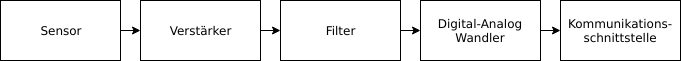
\includegraphics[width=\textwidth]{daq}

\paragraph{} Ansteuern von I2C Sensoren durch bitbanging
https://calcium3000.wordpress.com/2016/08/19/i2c-bit-banging-tutorial-part-i/

\subsection{Inertial Measurement Unit}
\paragraph{} Eine IMU enthält ein x-y-z Beschläunigunssensor und x-y-z
Gyroskop. Dient zur Assistierung der Bilderkennung und der Distanz
Messungen. Auch wenn schlussendlich keine IMU benötigt wird ist es trotzdem
ratsam eine zu verbauen, da es schlecht nachträglich hinzugefügt werden kann.

\paragraph{} Mögliche Kandidaten:
\begin{itemize}
\item LSM6DS3US
\item Kommunikationsinterface: I2C oder SPI
\item Stuckpreis: 3 CHF
\item Datenblatt: http://www.st.com/content/ccc/resource/technical/document/datasheet/group0/2e/84/27/34/60/8d/49/f2/DM00237513/files/DM00237513.pdf/jcr:content/translations/en.DM00237513.pdf
\end{itemize}

\subsection{Distanz Sensoren}
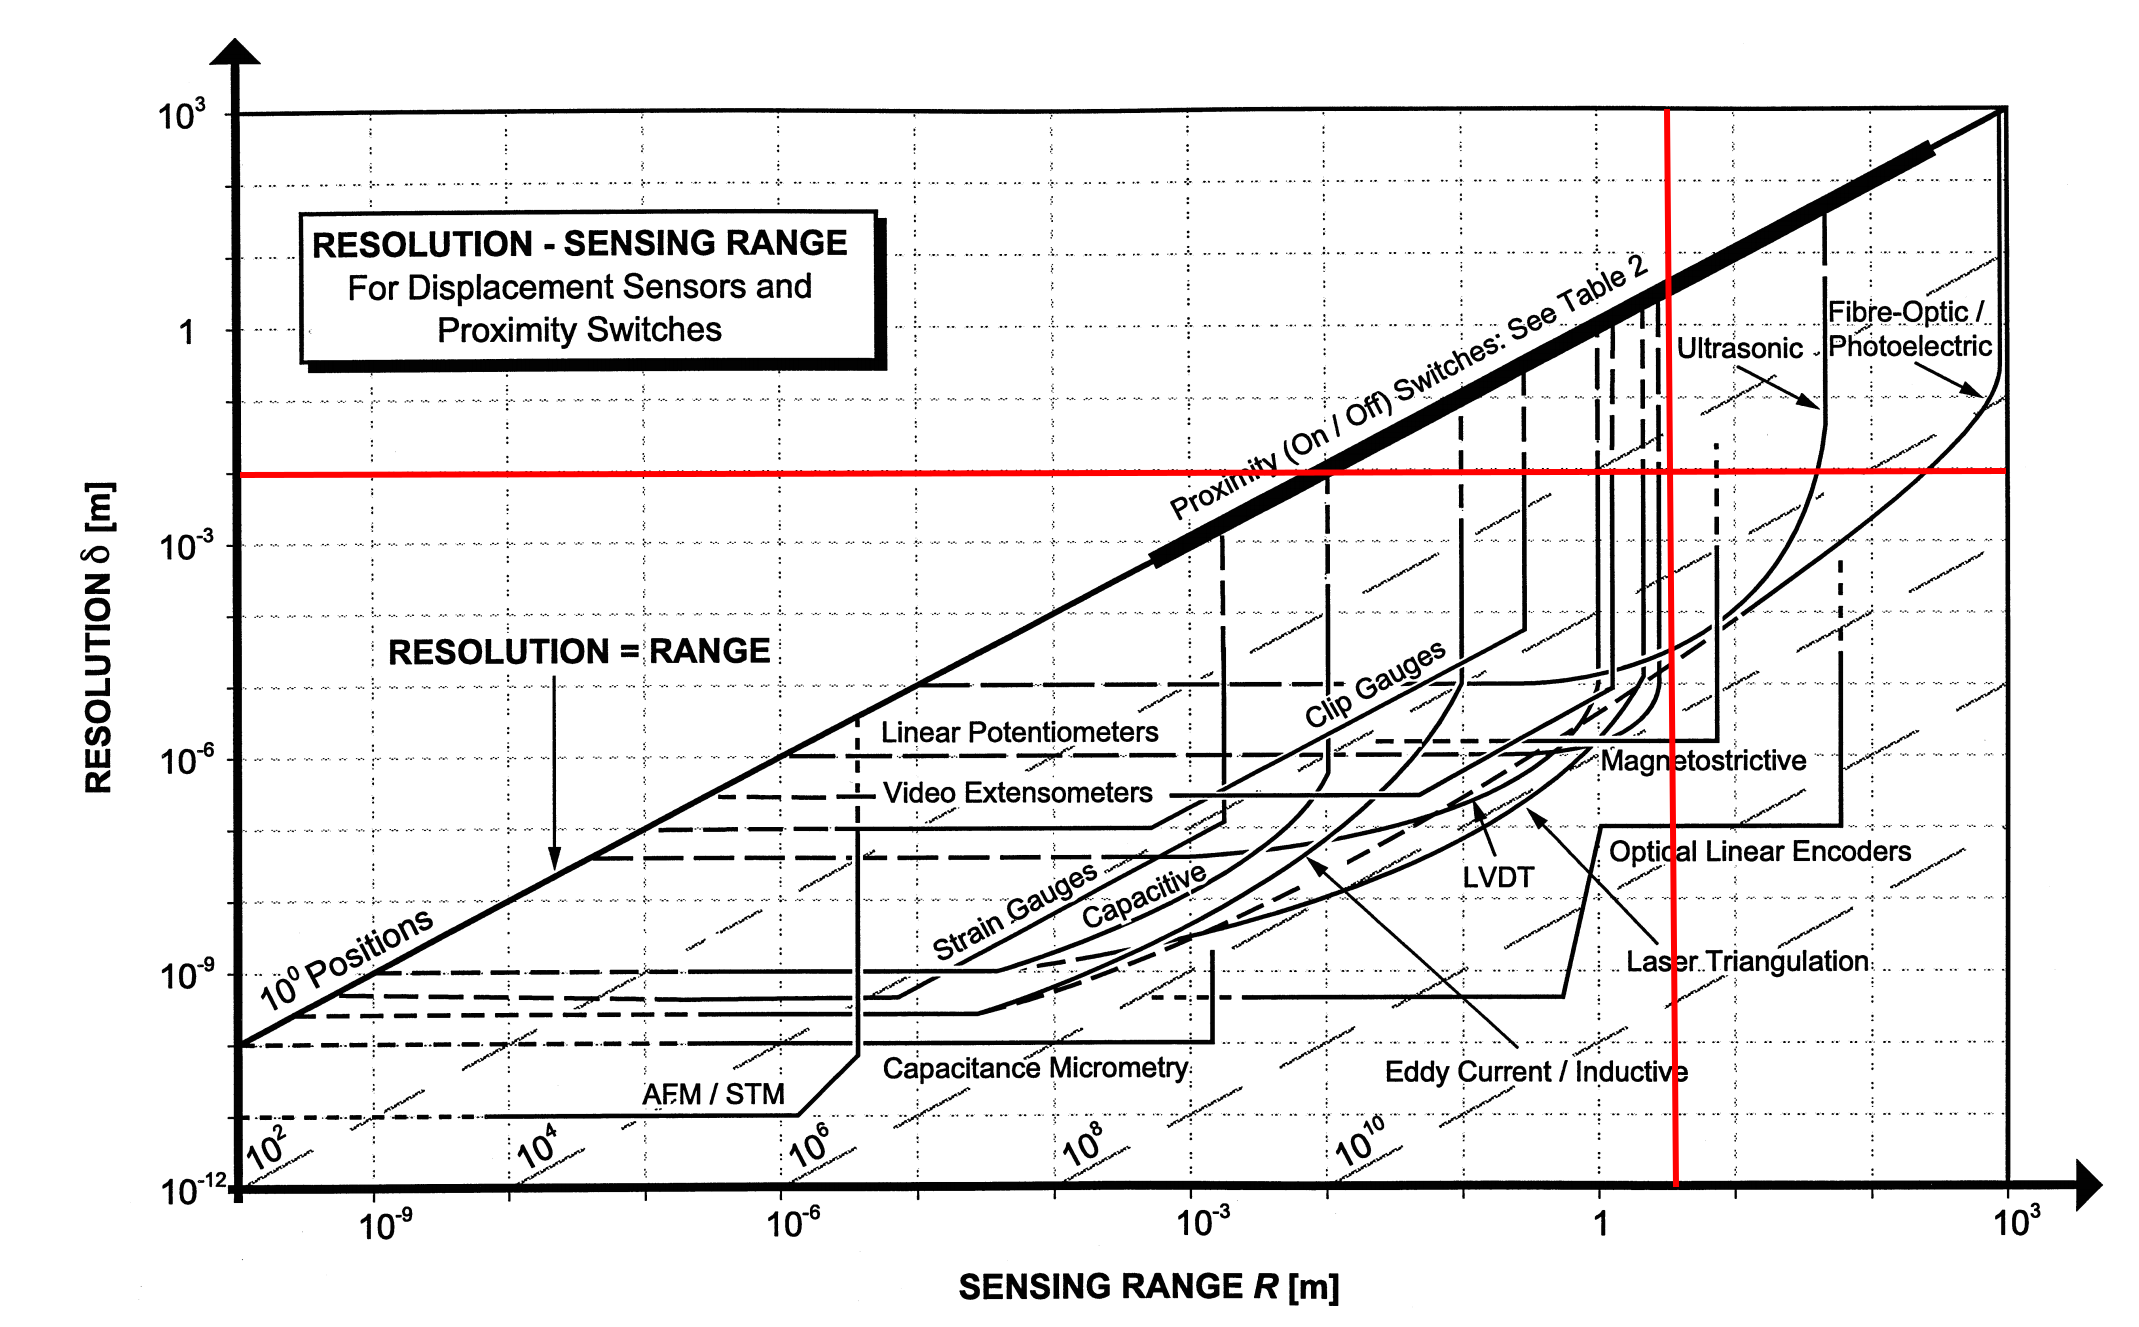
\includegraphics[width=\textwidth]{distance-sensors}

\paragraph{} Daraus schliessen wir das Ultraschall oder Photoelektrische
Sensoren für unsere Anwendung am besten geeignet sind.

\paragraph{} Sensor wahl - Was gibt es zu beachten:
http://www-mech.eng.cam.ac.uk/profiles/fleck/papers/134.pdf

\subsubsection{Distanz Messung in Z-Richtung}
\paragraph{} Assistieren der Bilderkennung beim erkennen von Hindernissen und
abschätzen der Z-Höhe des Ladegutes. Je nach dem was für einen Motor gewählt
wird kann dieser zur Abschätzung beitragen wie auch der Beschläunigunssensor
in Z-Richtung. Je nach grösse der Schwankungen in Y-Richtung kann das Gyroskop
in Y-Richtung auch zur prezise Messung beitragen.

\paragraph{} Anforderungen
\begin{itemize}
\item Reichweite: 60cm-110cm
\item Genauigkeit: 1cm
\end{itemize}

\paragraph{} Mögliche Kandidaten:
\begin{itemize}
\item Kandidat: VCNL4200
\item Kommunikationsinterface: I2C
\item Stuckpreis: 3 CHF
\item Datenblatt: https://www.vishay.com/optical-sensors/list/product-84430/
\end{itemize}

\subsubsection{Distanz Messung in X-Richtung}
\paragraph{} Genaue Positionsbestimmung auf der X-Achse.
\paragraph{} Mögliche Lösungsansätze (oder Kombination von Lösungsansätze) zu
evaluieren
\begin{itemize}
\item Ultraschall oder Photoelektrische Sensoren, obwohl aufgrund der Zeichnung das fehlen einer schönen Fläche vorne oder hinten zum Problem werden könnte.
\item Positionsbestimmung durch messen abgefahrener Strecke
\item Positionsbestimmung durch messen der Beschläunigung in X-Richtung
\item Positionsbestimmung durch Feature-Tracking
\end{itemize}

\subsection{Kamera}

\subsubsection{Optik}
\begin{itemize}
\item field of view
\item depth of field
\end{itemize}

\subsubsection{Bild Sensor}
\begin{itemize}
\item shutter speed (exposure time)
\item sampling pitch (higher resolution means less light sensitivity)
\item fill factor (spacing of photosensitive elements in camera sensor)
\item chip size
\item analog gain
\item sensor noise
\item resolution and noise of A/D
\end{itemize}

\subsection{Multisensor Data Fusion}
\paragraph{} Kalman filter - werden verwendet um aus unterschidlichen Messwerte aus
verschiedenen Quellen die best mögliche Schätzung zu erstellen:
http://bilgin.esme.org/BitsAndBytes/KalmanFilterforDummies

Multisensor Data Fusion: An Introduction

\section{User Interface}
\subsection{LCD}
\subsection{Misc}


\chapter{Lösungskonzept / Grobkonzept}
TODO Testat 2
Zusammensetzen verschiedener recherchierter Technologien zu Gesamtkonzepten. Diese Konzepte dann beurteilen und eines wählen.

\chapter{Schlussdiskussion}

\chapter{Verzeichnisse}
TODO Abbildungs-, Tabellen-, Formel-, Quellenverzeichnisse
\printbibliography

\chapter{Anhang}
\section{Meilensteinberichte}

\section{Task-Listen}

\end{document}
